% 高一13_复附浦东_周末作业2.tex —— 高一上数学「2026-2027 年复附浦东高一上周末作业 2」（试卷版/答案版）
% 试卷版：xelatex 高一13_复附浦东_周末作业2.tex
% 答案版：xelatex "\def\isanswer{1}% 高一13_复附浦东_周末作业2.tex —— 高一上数学「2026-2027 年复附浦东高一上周末作业 2」（试卷版/答案版）
% 试卷版：xelatex 高一13_复附浦东_周末作业2.tex
% 答案版：xelatex "\def\isanswer{1}% 高一13_复附浦东_周末作业2.tex —— 高一上数学「2026-2027 年复附浦东高一上周末作业 2」（试卷版/答案版）
% 试卷版：xelatex 高一13_复附浦东_周末作业2.tex
% 答案版：xelatex "\def\isanswer{1}% 高一13_复附浦东_周末作业2.tex —— 高一上数学「2026-2027 年复附浦东高一上周末作业 2」（试卷版/答案版）
% 试卷版：xelatex 高一13_复附浦东_周末作业2.tex
% 答案版：xelatex "\def\isanswer{1}\input{高一13_复附浦东_周末作业2.tex}"
%
% 原始材料是微信公众号图文（公众号「破晓」），正文为 7 张 PNG 页；原文本身就是一份**讲评版**
% ——题目下方直接印出【答案】或【解析】。试题文字、答案与解析均照原卷录入，未改内容。
%
% 与原卷的排版差异（均已在 README「说明」中交代）：
%   ① 原文自**第 3 题**起（第 1、2 题未在该文中发布），故本稿题号亦自 3 起；
%   ② 原卷未印分节标题，本稿按题型补「一、填空题 / 二、选择题 / 三、解答题」三节；
%   ③ 原卷填空、选择的答案直接印在题目下方（第 14 题更是直接印在括注里），本稿统一改为
%      试卷版隐去、答案版以【答案】给出，使两版彻底分离；
%   ④ 原卷的实数集符号时作正体 $R$、时作粗体 $\mathbf{R}$（第 14 题 D 选项与第 21 题均为粗体），
%      本稿按全稿惯例统一写作 $\R$.
%
% 原卷笔误三处（已逐处放大到能看清字形后核对，本稿按文意订正，并在 README 中写明原委）：
%   ① 第 10 题【解析】①、③ 两行原卷印作「①为真命题」「③为真命题」，与同段结论
%      「故真命题的是②④」以及两行自己给出的反例（9 是合数却不是偶数；$a=0$ 时方程无解）
%      都矛盾，显系笔误，本稿订正为「为假命题」；
%   ② 第 19(2) 中 $B=\{0\}$ 一行原卷印作 $a^2-1=-4\times(-4)$（与下一行 $B=\{-4\}$ 一字不差），
%      按两根均为 0 之积应为 0，本稿订正为 $a^2-1=0$——原卷紧接的「解得 $a=-1$」也只在
%      $a^2-1=0$ 下成立（注：同一道题在《高一07 交附闵行周练1》中原样抄录，此处按文意订正）；
%   ③ 第 19(1)【解析】列举子集时原卷印作「$\{0-4\}$」，漏排逗号，本稿写作 $\{0,-4\}$.

\documentclass[a4paper,11pt]{article}
\usepackage{common}

\begin{document}

\examtitlest[3]{2026--2027 年复附浦东高一上周末作业 2}{集合与常用逻辑用语}

\bigsec{一、填空题}

\begin{enumerate}
\setcounter{enumi}{2}

\item 已知集合 $A=\{2,a\}$，且 $1\in A$，则 $a=$ \blankline[2.4em].

\ans{$1$}

\item 集合 $A=\{x\mid x^2=1\}$，$B=\{x\mid x^2+x=0\}$，则 $A\cap B=$ \blankline[4.4em].

\ans{$\{-1\}$}

\ifanswer
\solbegin
\step{集合 $A=\{x\mid x^2=1\}=\{-1,1\}$，$B=\{x\mid x^2+x=0\}=\{-1,0\}$，}
\step{由交集定义得 $A\cap B=\{-1\}$.}
\solend

\fi

\item 已知集合 $A=\{1,3,5\},B=\{2,3,6\}$，则 $A\cup B=$ \blankline[4.4em].

\ans{$\{1,2,3,5,6\}$}

\item 若全集 $U=\R$，集合 $A=\{0,1,2,3,4\}$，$B=\{x\mid x>2\}$，则右图中阴影部分表示的集合为 \blankline[4.4em].

\begin{center}
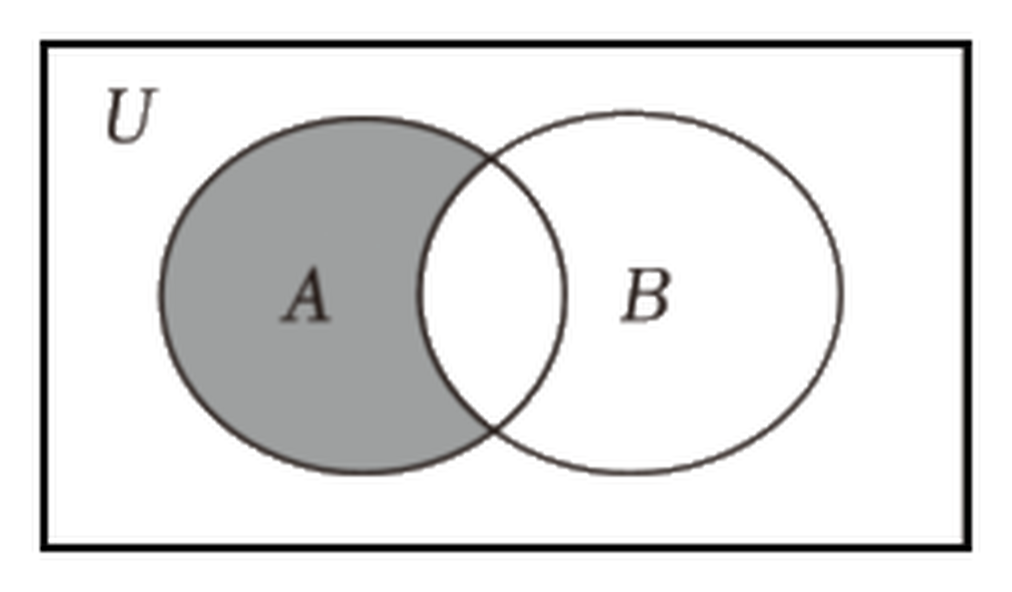
\includegraphics[width=0.34\textwidth]{figures/venn_A_minus_B.png}
\end{center}

\ans{$\{0,1,2\}$}

\ifanswer
\solbegin
\step{图中阴影部分表示的集合为 $A\cap\overline{B}=\{0,1,2\}$.}
\solend

\fi

\item 集合 $\{(x,y)\mid x+2y=2,\ x,y\in\N\}$ 用列举法表示为 \blankline[4.4em].

\ans{$\{(0,1),(2,0)\}$}

\ifanswer
\solbegin
\step{由题意得 $x+2y=2$ 可化为 $y=1-\dfrac{x}{2}$，}
\step{由 $y\in\N$，有 $y=1-\dfrac{x}{2}\geqslant 0$，解得 $x\leqslant 2$，}
\step{又由 $x\in\N$，得 $x$ 可能取值为 $0$，$1$，$2$，}
\step{当 $x=0$ 时，得 $y=1$，满足条件，}
\step{当 $x=1$ 时，得 $y=\dfrac{1}{2}\notin\N$，不满足条件，}
\step{当 $x=2$ 时，得 $y=0$，满足条件，}
\step{综上，集合用列举法表示为 $\{(0,1),(2,0)\}$.}
\solend

\fi

\item 若 $A=\{x\mid x=a^2+2a+4,\ a\in\R\}$，$B=\{y\mid y=b^2-4b+3,\ b\in\R\}$，则 $A$ 与 $B$ 的关系为 \blankline[4.4em].

% 注：此处符号为 $\subset$（真包含，无下划线；与第 10 题②、第 12 题、第 17 题等的
%     带下划线 $\subseteq$ 在卷面上明显不同，已逐处放大比对确认）。
\ans{$A\subset B$}

\ifanswer
\solbegin
\step{由 $x=a^2+2a+4=(a+1)^2+3$，}
\step{所以 $x=(a+1)^2+3\geqslant 3$，因此 $A=[3,+\infty)$，}
\step{由 $y=b^2-4b+3=(b-2)^2-1$，因为 $b\in\R$，所以 $y=(b-2)^2-1\geqslant -1$，}
\step{因此 $B=[-1,+\infty)$，因此 $A\subset B$.}
\solend

\fi

\item 在用反证法证明某命题时，对结论“$a,b,c$ 至少有一个为整数”的否定为 \blankline[4.4em].

\ans{$a,b,c$ 都不是整数}

\item 下列命题：①合数一定是偶数，②若 $A\cup B=B$，则 $A\sub B$，③方程 $ax+1=0$ 的解是 $x=-\dfrac{1}{a}$，④“$ac=bc$”是“$a=b$”的必要非充分条件，其中真命题的是 \blankline[2.4em]（填写序号）.

\ans{②④}

\ifanswer
\solbegin
% 注：以下 ①、③ 两行原卷印作「①为真命题」「③为真命题」，与两行自己给出的反例以及本段
%     末句「故真命题的是②④」都矛盾，系原卷笔误；本稿按文意订正为「为假命题」（结论不变）。
\step{对于①，$9$ 是合数，不是偶数，①为假命题；}
\step{对于②，由 $A\cup B=B$，得 $A\sub B$，②为真命题；}
\step{对于③，当 $a=0$ 时，$ax+1=0$ 无解，③为假命题；}
\step{对于④，当 $c=0$，$a=1$，$b=2$ 时满足 $ac=bc$，但 $a\neq b$，}
\step{当 $a=b$ 时，得 $ac=bc$，则“$ac=bc$”是“$a=b$”的必要非充分条件，}
\step{④为真命题.}
\step{故真命题的是②④.}
\solend

\fi

\item 设 $\alpha:4\leqslant x\leqslant 8$，$\beta:m+1\leqslant x\leqslant 2m+4$，$m\in\R$，$\alpha$ 是 $\beta$ 的充分不必要条件，则实数 $m$ 的取值范围是 \blankline[4.4em].

\ans{$[2,3]$}

\ifanswer
\solbegin
\step{因为 $\alpha$ 是 $\beta$ 的充分不必要条件，所以 $\begin{cases}m+1\leqslant 4\\ 2m+4\geqslant 8\end{cases}$，且等号不能同时成立，}
\step{解得 $2\leqslant m\leqslant 3$，所以实数 $m$ 的取值范围是 $[2,3]$.}
\solend

\fi

\item 已知集合 $A=\{a_1,a_2,\cdots,a_7\}$ 且 $A\sub\R$，定义 $\varphi(A)=\{a_ia_j\mid a_i,a_j\in A,\ 1\leqslant i<j\leqslant 7\}$，则 $\varphi(A)$ 的元素个数的最小值是 \blankline[2.4em].

\ans{$9$}

\ifanswer
\solbegin
\step{考虑等比数列，取 $A=\{-4,-2,-1,0,1,2,4\}$，}
\step{$\varphi(A)=\{8,4,0,-4,-8,-16,2,-2,-1\}$，元素个数最小值是 $9$.}
\solend

\fi

\end{enumerate}

\bigsec{二、选择题}

\begin{enumerate}
\setcounter{enumi}{12}

\item 已知 $M=\{(x,y)\mid x=y,\ x\in\R\}$，$N=\{(x,y)\mid y=x^2,\ x\in\R\}$，则 $M\cap N=$（\quad）.

A. $\{x\mid x\geqslant 0\}$\qquad B. $\{x\mid x\in\R\}$\qquad C. $\{(1,1)\}$\qquad D. $\{(1,1),(0,0)\}$

\ans{D}

\ifanswer
\solbegin
\step{联立方程组 $\begin{cases}x=y\\ y=x^2\end{cases}$，解得 $\begin{cases}x=0\\ y=0\end{cases}$ 或 $\begin{cases}x=1\\ y=1\end{cases}$，}
\step{则交点为 $(1,1)$、$(0,0)$，得到 $M\cap N=\{(1,1),(0,0)\}$. 故选 D.}
\solend

\fi

\item 下列说法中，正确的是（\quad）.

A. “$x>1$ 或 $y>1$”的否定形式是“$x\leqslant 1$ 或 $y\leqslant 1$”

B. “$1<x<3$”的否定形式是“$x<1$ 或 $x>3$”

C. “$\triangle ABC$ 是锐角三角形”的否定形式是“$\triangle ABC$ 中存在一个内角大于 $90^\circ$”

D. “任意 $x\in\R$，$f(x)=f(-x)$”的否定形式是“存在 $x_0\in\R$，使得 $f(x_0)\neq f(-x_0)$”

\ans{D}

\item 已知 $m,n$ 是非零自然数，命题 $\alpha:mn$ 是奇数，命题 $\beta:m$ 或 $n$ 是奇数，则 $\alpha$ 是 $\beta$ 的（\quad）

A. 充分非必要条件\qquad B. 必要非充分条件

C. 充要条件\qquad D. 既非充分又非必要条件

\ans{A}

\ifanswer
\solbegin
\step{$mn$ 是奇数 $\Leftrightarrow$ $m$、$n$ 都是奇数，所以 $\alpha$ 能推出 $\beta$，充分性成立，}
\step{但 $\beta$ 推不出 $\alpha$，必要性不成立，所以 $\alpha$ 是 $\beta$ 的充分非必要条件. 故选 A.}
\solend

\fi

\item 设 $k\geqslant 1,k\in\N$，已知集合 $M=\{1,2,3,4,5\}$，若集合 $N_1,N_2,\cdots,N_k$ 是集合 $M$ 的 $k$ 个不同非空子集，且 $N_1\cup N_2\cup\cdots\cup N_k\neq M$，则 $k$ 的最大值为（\quad）

A. $15$\qquad B. $16$\qquad C. $31$\qquad D. $32$

\ans{A}

\ifanswer
\solbegin
\step{由 $N_1\cup N_2\cup\cdots\cup N_k\neq M$ 得所有非空子集的并集缺少集合 $M$ 中至少一个元素，}
\step{假设缺少元素 $1$，则所有非空子集 $N_i$ 均不含元素 $1$，}
\step{即 $N_i$ 是集合 $\{2,3,4,5\}$ 非空子集，集合 $\{2,3,4,5\}$ 的非空子集个数为 $2^4-1=15$，}
\step{且这些子集 $N_i$ 的并集必不含 $1$，满足条件.}
\step{假设 $k\geqslant 16$，要满足所有非空子集的并集不等于集合 $M$，}
\step{必须至少有一个集合 $M$ 中的元素不在任何一个子集中，否则并集就会等于 $M$，}
\step{设这个缺失的元素是 $1$，那么 $k$ 个非空子集都不含元素 $1$，}
\step{即每个子集都是集合 $\{2,3,4,5\}$ 的非空子集，}
\step{而集合 $\{2,3,4,5\}$ 只有 $2^4-1=15$ 个不同的非空子集，}
\step{所以无法从中取出至少 $16$ 个不同的非空子集，}
\step{因此假设不成立，$k$ 必须小于 $16$，所以 $k$ 的最大值为 $15$，故选 A.}
\solend

\fi

\end{enumerate}

\bigsec{三、解答题}

\begin{enumerate}
\setcounter{enumi}{16}

\item 已知集合 $A=\{x\mid m-1\leqslant x\leqslant m+1\},B=\{x\mid x\leqslant 4\}$.

\begin{enumerate}[label=(\arabic*)]
\item 当 $m=4$ 时，求集合 $A\cap\overline{B}$；
\item 若“$x\in A$”是“$x\in B$”成立的充分非必要条件，求实数 $m$ 的取值范围.
\end{enumerate}

\ans{(1) $\{x\mid 4<x\leqslant 5\}$；（2）$\{m\mid m\leqslant 3\}$}

\ifanswer
\solbegin
\stepm{(1)}{当 $m=4$ 时，$A=\{x\mid 3\leqslant x\leqslant 5\}$，$\overline{B}=\{x\mid x>4\}$，}
\step{所以 $A\cap\overline{B}=\{x\mid 4<x\leqslant 5\}$.}
\stepm{(2)}{因为“$x\in A$”是“$x\in B$”成立的充分非必要条件，}
\step{所以 $A\sub B$，且 $B\neq A$，}
\step{易得 $A=\{x\mid m-1\leqslant x\leqslant m+1\}\neq\varnothing$，所以 $m+1\leqslant 4$，解得 $m\leqslant 3$，}
\step{符合题意；}
\step{综上所述，$m$ 的取值范围为 $\{m\mid m\leqslant 3\}$.}
\solend

\fi

\ansspace[7]

\item 设 $x\in\Z,a=x+5,b=20-x$.

\begin{enumerate}[label=(\arabic*)]
\item 求证：$a\neq b$；
\item 若 $c\in\Z$，求证：$c+a,c+b$ 中至少有一个数是奇数.
\end{enumerate}

\ans{(1) 略；（2）略}

\ifanswer
\solbegin
\stepm{(1)}{假设 $a=b$，则 $x+5=20-x\Rightarrow x=\dfrac{15}{2}\notin\Z$，与 $x\in\Z$ 矛盾，}
\step{则假设不成立，故 $a\neq b$.}
\stepm{(2)}{假设 $c+a,c+b$ 中都是偶数，}
\step{则 $c+a=c+x+5=2k_1,c+b=c+20-x=2k_2$，}
\step{两式相加并整理，得 $c=k_1+k_2-\dfrac{25}{2}\notin\Z$，与 $c\in\Z$ 矛盾，故假设不成立，}
\step{则 $c+a,c+b$ 中至少有一个数是奇数.}
\solend

\fi

\ansspace[8]

\item 设集合 $A=\{x\mid x^2+4x=0\}$，$B=\{x\mid x^2+2(a+1)x+a^2-1=0\}$.

\begin{enumerate}[label=(\arabic*)]
\item 写出集合 $A$ 的所有子集；
\item 若 $A\cap B=B$，求实数 $a$ 的取值范围.
\end{enumerate}

\ans{(1) $\varnothing,\{0\},\{-4\},\{0,-4\}$；（2）$a=1$ 或 $a\leqslant -1$}

\ifanswer
\solbegin
% 注：原卷此处列举子集时印作「$\{0-4\}$」，漏排逗号，本稿写作 $\{0,-4\}$.
\stepm{(1)}{由题意得 $A=\{0,-4\}$，集合 $A$ 的所有子集为 $\varnothing,\{0\},\{-4\},\{0,-4\}$；}
\stepm{(2)}{由 $A\cap B=B$ 得 $B\sub A$，}
\step{所以 $B=\{0\}$ 或 $B=\{-4\}$ 或 $B=\{0,-4\}$ 或 $B=\varnothing$，}
% 注：下面 $B=\{0\}$ 一行的两根之积，原卷印作 $a^2-1=-4\times(-4)$（与再下一行 $B=\{-4\}$
%     一字不差），按两根均为 0 之积应为 0；且原卷紧随的「解得 $a=-1$」也只在 $a^2-1=0$ 下成立，
%     故本稿订正为 $a^2-1=0$.
\step{若 $B=\{0\}$ 时，$x^2+2(a+1)x+a^2-1=0$ 有两个相等的根 $0$，}
\step{则 $\begin{cases}-2(a+1)=0\\ a^2-1=0\end{cases}$，解得 $a=-1$，}
\step{若 $B=\{-4\}$ 时，$x^2+2(a+1)x+a^2-1=0$ 有两个相等的根 $-4$，}
\step{则 $\begin{cases}-2(a+1)=-8\\ a^2-1=-4\times(-4)\end{cases}$，$a$ 无解，}
\step{若 $B=\{0,-4\}$ 时，$x^2+2(a+1)x+a^2-1=0$ 有两个不相等的根 $0$ 和 $-4$，}
\step{则 $\begin{cases}-2(a+1)=-4\\ a^2-1=0\end{cases}$，解得 $a=1$，}
\step{当 $B=\varnothing$ 时，$x^2+2(a+1)x+a^2-1=0$ 无实数根，}
\step{$\Delta=[2(a+1)]^2-4(a^2-1)=8a+8<0$，得 $a<-1$.}
\step{综上，$a=1$ 或 $a\leqslant -1$.}
\solend

\fi

\ansspace[8]

\item 已知集合 $A=\{x\mid x<-2\text{ 或 }x\geqslant 3\}$，$U=\R$.

\begin{enumerate}[label=(\arabic*)]
\item 求 $\overline{A}$；
\item 若 $B=\{x\mid mx-1>0\}$，当 $B\sub A$ 时，求实数 $m$ 的取值范围；
\item 若 $B=\{x\mid 2m-6\leqslant x\leqslant m+4\}$，当 $B\cap\overline{A}=\varnothing$ 时，求实数 $m$ 的取值范围.
\end{enumerate}

\ans{(1) $\{x\mid -2\leqslant x<3\}$；（2）$\left[-\dfrac{1}{2},\dfrac{1}{3}\right]$；（3）$(-\infty,-6)\cup\left[\dfrac{9}{2},+\infty\right)$}

\ifanswer
\solbegin
\stepm{(1)}{因为集合 $A=\{x\mid x<-2\text{ 或 }x\geqslant 3\}$，$U=\R$，所以 $\overline{A}=\{x\mid -2\leqslant x<3\}$；}
\stepm{(2)}{当 $m=0$ 时，$B=\varnothing$，符合题意，}
\step{当 $m>0$ 时，$B=\left\{x\mid x>\dfrac{1}{m}\right\}$，则 $\dfrac{1}{m}\geqslant 3$，解得 $0<m\leqslant\dfrac{1}{3}$，}
\step{当 $m<0$ 时，$B=\left\{x\mid x<\dfrac{1}{m}\right\}$，则 $\dfrac{1}{m}\leqslant -2$，解得 $-\dfrac{1}{2}\leqslant m<0$，}
\step{综上所述，实数 $m$ 的取值范围 $\left[-\dfrac{1}{2},\dfrac{1}{3}\right]$；}
\stepm{(3)}{由题意得 $B=\{x\mid 2m-6\leqslant x\leqslant m+4\}$，$\overline{A}=\{x\mid -2\leqslant x<3\}$，且 $B\cap\overline{A}=\varnothing$，}
\step{当 $B=\varnothing$ 时，$2m-6>m+4$，解得 $m>10$，}
\step{当 $B\neq\varnothing$ 时，则 $\begin{cases}2m-6\leqslant m+4\\ m+4<-2\end{cases}$ 或 $\begin{cases}2m-6\leqslant m+4\\ 2m-6\geqslant 3\end{cases}$，}
\step{解得 $m<-6$ 或 $\dfrac{9}{2}\leqslant m\leqslant 10$，}
\step{综上所述，实数 $m$ 的取值范围为 $(-\infty,-6)\cup\left[\dfrac{9}{2},+\infty\right)$.}
\solend

\fi

\ansspace[10]

% 压轴题：其后已无内容，故作答区全用可丢弃胶水（\ansspace*），并在题目前先量一下版面。
\ansneed{7cm}

\item 给定数集 $M$，若对于任意 $a$、$b\in M$，有 $a+b\in M,a-b\in M$，则称集合 $M$ 为闭集合.

\begin{enumerate}[label=(\arabic*)]
\item 判断集合 $A_1=\{-4,-2,0,2,4\}$，集合 $B=\{x\mid x=3k,k\in\Z\}$ 是否为闭集合；
\item 若集合 $C$、$D$ 为闭集合，则 $C\cup D$ 是否一定为闭集合？请说明理由；
\item 已知集合 $C$、$D$ 为闭集合，且 $C\subset\R,D\subset\R$，证明：$(C\cup D)\subset\R$.
\end{enumerate}

\ans{(1) $A_1$ 不是闭集合，$B$ 是闭集合；（2）不一定；（3）略}

\ifanswer
\solbegin
\stepm{(1)}{因为 $4\in A_1,2\in A_1,4+2=6\notin A_1$，所以 $A_1$ 不是闭集合；}
\step{任取 $x,y\in B$，设 $x=3m,y=3n,m,n\in\Z$，}
\step{则 $x+y=3m+3n=3(m+n)$ 且 $m+n\in\Z$，}
\step{所以 $x+y\in B$，同理，$x-y\in B$，故 $B$ 为闭集合.}
\stepm{(2)}{结论：不一定.}
\step{不妨令 $C=\{x\mid x=2k,k\in\Z\},D=\{x\mid x=3k,k\in\Z\}$，}
\step{则由（1）得 $C$、$D$ 为闭集合，易得 $2,3\in C\cup D,2+3=5\notin C\cup D$，}
\step{因此，$C\cup D$ 不一定是闭集合.}
\stepm{(3)}{不妨假设 $C\cup D=\R$，则由 $C\subset\R$，得存在 $a\in\R$ 且 $a\notin C$，故 $a\in D$.}
\step{同理，存在 $b\in\R$ 且 $b\notin D$，故 $b\in C$.}
\step{因为 $a+b\in\R=C\cup D$，所以 $a+b\in C$ 或 $a+b\in D$.}
\step{若 $a+b\in C$，则由 $C$ 为闭集合且 $b\in C$，得 $a=(a+b)-b\in C$，}
\step{与 $a\notin C$ 矛盾.}
\step{若 $a+b\in D$，则由 $D$ 为闭集合且 $a\in D$，得 $b=(a+b)-a\in D$，}
\step{与 $b\notin D$ 矛盾.}
\step{综上，$C\cup D=\R$ 不成立，故 $(C\cup D)\subset\R$.}
\solend

\fi

\ansspace*[12]

\end{enumerate}

\end{document}
"
%
% 原始材料是微信公众号图文（公众号「破晓」），正文为 7 张 PNG 页；原文本身就是一份**讲评版**
% ——题目下方直接印出【答案】或【解析】。试题文字、答案与解析均照原卷录入，未改内容。
%
% 与原卷的排版差异（均已在 README「说明」中交代）：
%   ① 原文自**第 3 题**起（第 1、2 题未在该文中发布），故本稿题号亦自 3 起；
%   ② 原卷未印分节标题，本稿按题型补「一、填空题 / 二、选择题 / 三、解答题」三节；
%   ③ 原卷填空、选择的答案直接印在题目下方（第 14 题更是直接印在括注里），本稿统一改为
%      试卷版隐去、答案版以【答案】给出，使两版彻底分离；
%   ④ 原卷的实数集符号时作正体 $R$、时作粗体 $\mathbf{R}$（第 14 题 D 选项与第 21 题均为粗体），
%      本稿按全稿惯例统一写作 $\R$.
%
% 原卷笔误三处（已逐处放大到能看清字形后核对，本稿按文意订正，并在 README 中写明原委）：
%   ① 第 10 题【解析】①、③ 两行原卷印作「①为真命题」「③为真命题」，与同段结论
%      「故真命题的是②④」以及两行自己给出的反例（9 是合数却不是偶数；$a=0$ 时方程无解）
%      都矛盾，显系笔误，本稿订正为「为假命题」；
%   ② 第 19(2) 中 $B=\{0\}$ 一行原卷印作 $a^2-1=-4\times(-4)$（与下一行 $B=\{-4\}$ 一字不差），
%      按两根均为 0 之积应为 0，本稿订正为 $a^2-1=0$——原卷紧接的「解得 $a=-1$」也只在
%      $a^2-1=0$ 下成立（注：同一道题在《高一07 交附闵行周练1》中原样抄录，此处按文意订正）；
%   ③ 第 19(1)【解析】列举子集时原卷印作「$\{0-4\}$」，漏排逗号，本稿写作 $\{0,-4\}$.

\documentclass[a4paper,11pt]{article}
\usepackage{common}

\begin{document}

\examtitlest[3]{2026--2027 年复附浦东高一上周末作业 2}{集合与常用逻辑用语}

\bigsec{一、填空题}

\begin{enumerate}
\setcounter{enumi}{2}

\item 已知集合 $A=\{2,a\}$，且 $1\in A$，则 $a=$ \blankline[2.4em].

\ans{$1$}

\item 集合 $A=\{x\mid x^2=1\}$，$B=\{x\mid x^2+x=0\}$，则 $A\cap B=$ \blankline[4.4em].

\ans{$\{-1\}$}

\ifanswer
\solbegin
\step{集合 $A=\{x\mid x^2=1\}=\{-1,1\}$，$B=\{x\mid x^2+x=0\}=\{-1,0\}$，}
\step{由交集定义得 $A\cap B=\{-1\}$.}
\solend

\fi

\item 已知集合 $A=\{1,3,5\},B=\{2,3,6\}$，则 $A\cup B=$ \blankline[4.4em].

\ans{$\{1,2,3,5,6\}$}

\item 若全集 $U=\R$，集合 $A=\{0,1,2,3,4\}$，$B=\{x\mid x>2\}$，则右图中阴影部分表示的集合为 \blankline[4.4em].

\begin{center}
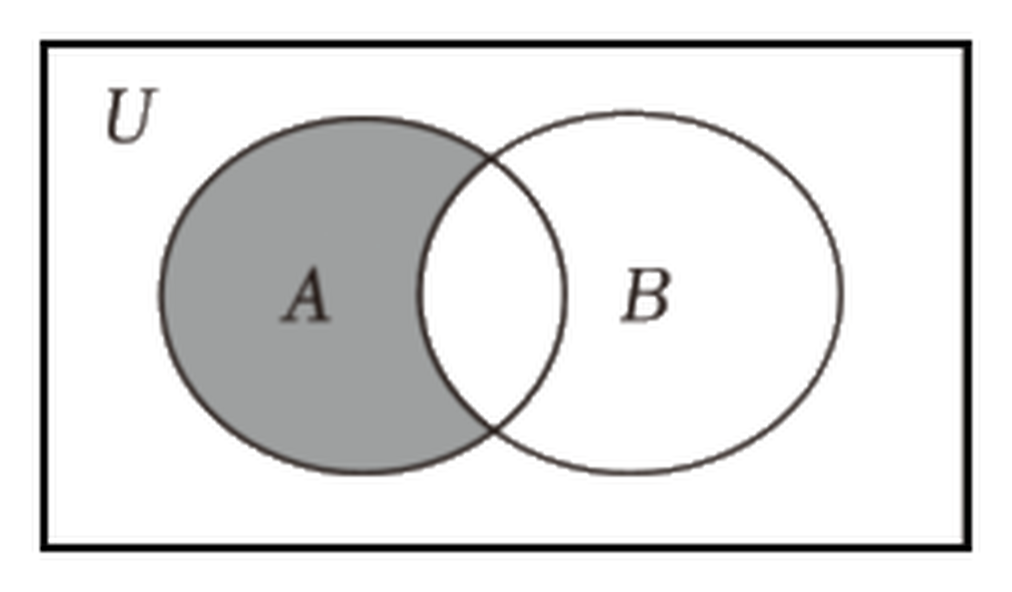
\includegraphics[width=0.34\textwidth]{figures/venn_A_minus_B.png}
\end{center}

\ans{$\{0,1,2\}$}

\ifanswer
\solbegin
\step{图中阴影部分表示的集合为 $A\cap\overline{B}=\{0,1,2\}$.}
\solend

\fi

\item 集合 $\{(x,y)\mid x+2y=2,\ x,y\in\N\}$ 用列举法表示为 \blankline[4.4em].

\ans{$\{(0,1),(2,0)\}$}

\ifanswer
\solbegin
\step{由题意得 $x+2y=2$ 可化为 $y=1-\dfrac{x}{2}$，}
\step{由 $y\in\N$，有 $y=1-\dfrac{x}{2}\geqslant 0$，解得 $x\leqslant 2$，}
\step{又由 $x\in\N$，得 $x$ 可能取值为 $0$，$1$，$2$，}
\step{当 $x=0$ 时，得 $y=1$，满足条件，}
\step{当 $x=1$ 时，得 $y=\dfrac{1}{2}\notin\N$，不满足条件，}
\step{当 $x=2$ 时，得 $y=0$，满足条件，}
\step{综上，集合用列举法表示为 $\{(0,1),(2,0)\}$.}
\solend

\fi

\item 若 $A=\{x\mid x=a^2+2a+4,\ a\in\R\}$，$B=\{y\mid y=b^2-4b+3,\ b\in\R\}$，则 $A$ 与 $B$ 的关系为 \blankline[4.4em].

% 注：此处符号为 $\subset$（真包含，无下划线；与第 10 题②、第 12 题、第 17 题等的
%     带下划线 $\subseteq$ 在卷面上明显不同，已逐处放大比对确认）。
\ans{$A\subset B$}

\ifanswer
\solbegin
\step{由 $x=a^2+2a+4=(a+1)^2+3$，}
\step{所以 $x=(a+1)^2+3\geqslant 3$，因此 $A=[3,+\infty)$，}
\step{由 $y=b^2-4b+3=(b-2)^2-1$，因为 $b\in\R$，所以 $y=(b-2)^2-1\geqslant -1$，}
\step{因此 $B=[-1,+\infty)$，因此 $A\subset B$.}
\solend

\fi

\item 在用反证法证明某命题时，对结论“$a,b,c$ 至少有一个为整数”的否定为 \blankline[4.4em].

\ans{$a,b,c$ 都不是整数}

\item 下列命题：①合数一定是偶数，②若 $A\cup B=B$，则 $A\sub B$，③方程 $ax+1=0$ 的解是 $x=-\dfrac{1}{a}$，④“$ac=bc$”是“$a=b$”的必要非充分条件，其中真命题的是 \blankline[2.4em]（填写序号）.

\ans{②④}

\ifanswer
\solbegin
% 注：以下 ①、③ 两行原卷印作「①为真命题」「③为真命题」，与两行自己给出的反例以及本段
%     末句「故真命题的是②④」都矛盾，系原卷笔误；本稿按文意订正为「为假命题」（结论不变）。
\step{对于①，$9$ 是合数，不是偶数，①为假命题；}
\step{对于②，由 $A\cup B=B$，得 $A\sub B$，②为真命题；}
\step{对于③，当 $a=0$ 时，$ax+1=0$ 无解，③为假命题；}
\step{对于④，当 $c=0$，$a=1$，$b=2$ 时满足 $ac=bc$，但 $a\neq b$，}
\step{当 $a=b$ 时，得 $ac=bc$，则“$ac=bc$”是“$a=b$”的必要非充分条件，}
\step{④为真命题.}
\step{故真命题的是②④.}
\solend

\fi

\item 设 $\alpha:4\leqslant x\leqslant 8$，$\beta:m+1\leqslant x\leqslant 2m+4$，$m\in\R$，$\alpha$ 是 $\beta$ 的充分不必要条件，则实数 $m$ 的取值范围是 \blankline[4.4em].

\ans{$[2,3]$}

\ifanswer
\solbegin
\step{因为 $\alpha$ 是 $\beta$ 的充分不必要条件，所以 $\begin{cases}m+1\leqslant 4\\ 2m+4\geqslant 8\end{cases}$，且等号不能同时成立，}
\step{解得 $2\leqslant m\leqslant 3$，所以实数 $m$ 的取值范围是 $[2,3]$.}
\solend

\fi

\item 已知集合 $A=\{a_1,a_2,\cdots,a_7\}$ 且 $A\sub\R$，定义 $\varphi(A)=\{a_ia_j\mid a_i,a_j\in A,\ 1\leqslant i<j\leqslant 7\}$，则 $\varphi(A)$ 的元素个数的最小值是 \blankline[2.4em].

\ans{$9$}

\ifanswer
\solbegin
\step{考虑等比数列，取 $A=\{-4,-2,-1,0,1,2,4\}$，}
\step{$\varphi(A)=\{8,4,0,-4,-8,-16,2,-2,-1\}$，元素个数最小值是 $9$.}
\solend

\fi

\end{enumerate}

\bigsec{二、选择题}

\begin{enumerate}
\setcounter{enumi}{12}

\item 已知 $M=\{(x,y)\mid x=y,\ x\in\R\}$，$N=\{(x,y)\mid y=x^2,\ x\in\R\}$，则 $M\cap N=$（\quad）.

A. $\{x\mid x\geqslant 0\}$\qquad B. $\{x\mid x\in\R\}$\qquad C. $\{(1,1)\}$\qquad D. $\{(1,1),(0,0)\}$

\ans{D}

\ifanswer
\solbegin
\step{联立方程组 $\begin{cases}x=y\\ y=x^2\end{cases}$，解得 $\begin{cases}x=0\\ y=0\end{cases}$ 或 $\begin{cases}x=1\\ y=1\end{cases}$，}
\step{则交点为 $(1,1)$、$(0,0)$，得到 $M\cap N=\{(1,1),(0,0)\}$. 故选 D.}
\solend

\fi

\item 下列说法中，正确的是（\quad）.

A. “$x>1$ 或 $y>1$”的否定形式是“$x\leqslant 1$ 或 $y\leqslant 1$”

B. “$1<x<3$”的否定形式是“$x<1$ 或 $x>3$”

C. “$\triangle ABC$ 是锐角三角形”的否定形式是“$\triangle ABC$ 中存在一个内角大于 $90^\circ$”

D. “任意 $x\in\R$，$f(x)=f(-x)$”的否定形式是“存在 $x_0\in\R$，使得 $f(x_0)\neq f(-x_0)$”

\ans{D}

\item 已知 $m,n$ 是非零自然数，命题 $\alpha:mn$ 是奇数，命题 $\beta:m$ 或 $n$ 是奇数，则 $\alpha$ 是 $\beta$ 的（\quad）

A. 充分非必要条件\qquad B. 必要非充分条件

C. 充要条件\qquad D. 既非充分又非必要条件

\ans{A}

\ifanswer
\solbegin
\step{$mn$ 是奇数 $\Leftrightarrow$ $m$、$n$ 都是奇数，所以 $\alpha$ 能推出 $\beta$，充分性成立，}
\step{但 $\beta$ 推不出 $\alpha$，必要性不成立，所以 $\alpha$ 是 $\beta$ 的充分非必要条件. 故选 A.}
\solend

\fi

\item 设 $k\geqslant 1,k\in\N$，已知集合 $M=\{1,2,3,4,5\}$，若集合 $N_1,N_2,\cdots,N_k$ 是集合 $M$ 的 $k$ 个不同非空子集，且 $N_1\cup N_2\cup\cdots\cup N_k\neq M$，则 $k$ 的最大值为（\quad）

A. $15$\qquad B. $16$\qquad C. $31$\qquad D. $32$

\ans{A}

\ifanswer
\solbegin
\step{由 $N_1\cup N_2\cup\cdots\cup N_k\neq M$ 得所有非空子集的并集缺少集合 $M$ 中至少一个元素，}
\step{假设缺少元素 $1$，则所有非空子集 $N_i$ 均不含元素 $1$，}
\step{即 $N_i$ 是集合 $\{2,3,4,5\}$ 非空子集，集合 $\{2,3,4,5\}$ 的非空子集个数为 $2^4-1=15$，}
\step{且这些子集 $N_i$ 的并集必不含 $1$，满足条件.}
\step{假设 $k\geqslant 16$，要满足所有非空子集的并集不等于集合 $M$，}
\step{必须至少有一个集合 $M$ 中的元素不在任何一个子集中，否则并集就会等于 $M$，}
\step{设这个缺失的元素是 $1$，那么 $k$ 个非空子集都不含元素 $1$，}
\step{即每个子集都是集合 $\{2,3,4,5\}$ 的非空子集，}
\step{而集合 $\{2,3,4,5\}$ 只有 $2^4-1=15$ 个不同的非空子集，}
\step{所以无法从中取出至少 $16$ 个不同的非空子集，}
\step{因此假设不成立，$k$ 必须小于 $16$，所以 $k$ 的最大值为 $15$，故选 A.}
\solend

\fi

\end{enumerate}

\bigsec{三、解答题}

\begin{enumerate}
\setcounter{enumi}{16}

\item 已知集合 $A=\{x\mid m-1\leqslant x\leqslant m+1\},B=\{x\mid x\leqslant 4\}$.

\begin{enumerate}[label=(\arabic*)]
\item 当 $m=4$ 时，求集合 $A\cap\overline{B}$；
\item 若“$x\in A$”是“$x\in B$”成立的充分非必要条件，求实数 $m$ 的取值范围.
\end{enumerate}

\ans{(1) $\{x\mid 4<x\leqslant 5\}$；（2）$\{m\mid m\leqslant 3\}$}

\ifanswer
\solbegin
\stepm{(1)}{当 $m=4$ 时，$A=\{x\mid 3\leqslant x\leqslant 5\}$，$\overline{B}=\{x\mid x>4\}$，}
\step{所以 $A\cap\overline{B}=\{x\mid 4<x\leqslant 5\}$.}
\stepm{(2)}{因为“$x\in A$”是“$x\in B$”成立的充分非必要条件，}
\step{所以 $A\sub B$，且 $B\neq A$，}
\step{易得 $A=\{x\mid m-1\leqslant x\leqslant m+1\}\neq\varnothing$，所以 $m+1\leqslant 4$，解得 $m\leqslant 3$，}
\step{符合题意；}
\step{综上所述，$m$ 的取值范围为 $\{m\mid m\leqslant 3\}$.}
\solend

\fi

\ansspace[7]

\item 设 $x\in\Z,a=x+5,b=20-x$.

\begin{enumerate}[label=(\arabic*)]
\item 求证：$a\neq b$；
\item 若 $c\in\Z$，求证：$c+a,c+b$ 中至少有一个数是奇数.
\end{enumerate}

\ans{(1) 略；（2）略}

\ifanswer
\solbegin
\stepm{(1)}{假设 $a=b$，则 $x+5=20-x\Rightarrow x=\dfrac{15}{2}\notin\Z$，与 $x\in\Z$ 矛盾，}
\step{则假设不成立，故 $a\neq b$.}
\stepm{(2)}{假设 $c+a,c+b$ 中都是偶数，}
\step{则 $c+a=c+x+5=2k_1,c+b=c+20-x=2k_2$，}
\step{两式相加并整理，得 $c=k_1+k_2-\dfrac{25}{2}\notin\Z$，与 $c\in\Z$ 矛盾，故假设不成立，}
\step{则 $c+a,c+b$ 中至少有一个数是奇数.}
\solend

\fi

\ansspace[8]

\item 设集合 $A=\{x\mid x^2+4x=0\}$，$B=\{x\mid x^2+2(a+1)x+a^2-1=0\}$.

\begin{enumerate}[label=(\arabic*)]
\item 写出集合 $A$ 的所有子集；
\item 若 $A\cap B=B$，求实数 $a$ 的取值范围.
\end{enumerate}

\ans{(1) $\varnothing,\{0\},\{-4\},\{0,-4\}$；（2）$a=1$ 或 $a\leqslant -1$}

\ifanswer
\solbegin
% 注：原卷此处列举子集时印作「$\{0-4\}$」，漏排逗号，本稿写作 $\{0,-4\}$.
\stepm{(1)}{由题意得 $A=\{0,-4\}$，集合 $A$ 的所有子集为 $\varnothing,\{0\},\{-4\},\{0,-4\}$；}
\stepm{(2)}{由 $A\cap B=B$ 得 $B\sub A$，}
\step{所以 $B=\{0\}$ 或 $B=\{-4\}$ 或 $B=\{0,-4\}$ 或 $B=\varnothing$，}
% 注：下面 $B=\{0\}$ 一行的两根之积，原卷印作 $a^2-1=-4\times(-4)$（与再下一行 $B=\{-4\}$
%     一字不差），按两根均为 0 之积应为 0；且原卷紧随的「解得 $a=-1$」也只在 $a^2-1=0$ 下成立，
%     故本稿订正为 $a^2-1=0$.
\step{若 $B=\{0\}$ 时，$x^2+2(a+1)x+a^2-1=0$ 有两个相等的根 $0$，}
\step{则 $\begin{cases}-2(a+1)=0\\ a^2-1=0\end{cases}$，解得 $a=-1$，}
\step{若 $B=\{-4\}$ 时，$x^2+2(a+1)x+a^2-1=0$ 有两个相等的根 $-4$，}
\step{则 $\begin{cases}-2(a+1)=-8\\ a^2-1=-4\times(-4)\end{cases}$，$a$ 无解，}
\step{若 $B=\{0,-4\}$ 时，$x^2+2(a+1)x+a^2-1=0$ 有两个不相等的根 $0$ 和 $-4$，}
\step{则 $\begin{cases}-2(a+1)=-4\\ a^2-1=0\end{cases}$，解得 $a=1$，}
\step{当 $B=\varnothing$ 时，$x^2+2(a+1)x+a^2-1=0$ 无实数根，}
\step{$\Delta=[2(a+1)]^2-4(a^2-1)=8a+8<0$，得 $a<-1$.}
\step{综上，$a=1$ 或 $a\leqslant -1$.}
\solend

\fi

\ansspace[8]

\item 已知集合 $A=\{x\mid x<-2\text{ 或 }x\geqslant 3\}$，$U=\R$.

\begin{enumerate}[label=(\arabic*)]
\item 求 $\overline{A}$；
\item 若 $B=\{x\mid mx-1>0\}$，当 $B\sub A$ 时，求实数 $m$ 的取值范围；
\item 若 $B=\{x\mid 2m-6\leqslant x\leqslant m+4\}$，当 $B\cap\overline{A}=\varnothing$ 时，求实数 $m$ 的取值范围.
\end{enumerate}

\ans{(1) $\{x\mid -2\leqslant x<3\}$；（2）$\left[-\dfrac{1}{2},\dfrac{1}{3}\right]$；（3）$(-\infty,-6)\cup\left[\dfrac{9}{2},+\infty\right)$}

\ifanswer
\solbegin
\stepm{(1)}{因为集合 $A=\{x\mid x<-2\text{ 或 }x\geqslant 3\}$，$U=\R$，所以 $\overline{A}=\{x\mid -2\leqslant x<3\}$；}
\stepm{(2)}{当 $m=0$ 时，$B=\varnothing$，符合题意，}
\step{当 $m>0$ 时，$B=\left\{x\mid x>\dfrac{1}{m}\right\}$，则 $\dfrac{1}{m}\geqslant 3$，解得 $0<m\leqslant\dfrac{1}{3}$，}
\step{当 $m<0$ 时，$B=\left\{x\mid x<\dfrac{1}{m}\right\}$，则 $\dfrac{1}{m}\leqslant -2$，解得 $-\dfrac{1}{2}\leqslant m<0$，}
\step{综上所述，实数 $m$ 的取值范围 $\left[-\dfrac{1}{2},\dfrac{1}{3}\right]$；}
\stepm{(3)}{由题意得 $B=\{x\mid 2m-6\leqslant x\leqslant m+4\}$，$\overline{A}=\{x\mid -2\leqslant x<3\}$，且 $B\cap\overline{A}=\varnothing$，}
\step{当 $B=\varnothing$ 时，$2m-6>m+4$，解得 $m>10$，}
\step{当 $B\neq\varnothing$ 时，则 $\begin{cases}2m-6\leqslant m+4\\ m+4<-2\end{cases}$ 或 $\begin{cases}2m-6\leqslant m+4\\ 2m-6\geqslant 3\end{cases}$，}
\step{解得 $m<-6$ 或 $\dfrac{9}{2}\leqslant m\leqslant 10$，}
\step{综上所述，实数 $m$ 的取值范围为 $(-\infty,-6)\cup\left[\dfrac{9}{2},+\infty\right)$.}
\solend

\fi

\ansspace[10]

% 压轴题：其后已无内容，故作答区全用可丢弃胶水（\ansspace*），并在题目前先量一下版面。
\ansneed{7cm}

\item 给定数集 $M$，若对于任意 $a$、$b\in M$，有 $a+b\in M,a-b\in M$，则称集合 $M$ 为闭集合.

\begin{enumerate}[label=(\arabic*)]
\item 判断集合 $A_1=\{-4,-2,0,2,4\}$，集合 $B=\{x\mid x=3k,k\in\Z\}$ 是否为闭集合；
\item 若集合 $C$、$D$ 为闭集合，则 $C\cup D$ 是否一定为闭集合？请说明理由；
\item 已知集合 $C$、$D$ 为闭集合，且 $C\subset\R,D\subset\R$，证明：$(C\cup D)\subset\R$.
\end{enumerate}

\ans{(1) $A_1$ 不是闭集合，$B$ 是闭集合；（2）不一定；（3）略}

\ifanswer
\solbegin
\stepm{(1)}{因为 $4\in A_1,2\in A_1,4+2=6\notin A_1$，所以 $A_1$ 不是闭集合；}
\step{任取 $x,y\in B$，设 $x=3m,y=3n,m,n\in\Z$，}
\step{则 $x+y=3m+3n=3(m+n)$ 且 $m+n\in\Z$，}
\step{所以 $x+y\in B$，同理，$x-y\in B$，故 $B$ 为闭集合.}
\stepm{(2)}{结论：不一定.}
\step{不妨令 $C=\{x\mid x=2k,k\in\Z\},D=\{x\mid x=3k,k\in\Z\}$，}
\step{则由（1）得 $C$、$D$ 为闭集合，易得 $2,3\in C\cup D,2+3=5\notin C\cup D$，}
\step{因此，$C\cup D$ 不一定是闭集合.}
\stepm{(3)}{不妨假设 $C\cup D=\R$，则由 $C\subset\R$，得存在 $a\in\R$ 且 $a\notin C$，故 $a\in D$.}
\step{同理，存在 $b\in\R$ 且 $b\notin D$，故 $b\in C$.}
\step{因为 $a+b\in\R=C\cup D$，所以 $a+b\in C$ 或 $a+b\in D$.}
\step{若 $a+b\in C$，则由 $C$ 为闭集合且 $b\in C$，得 $a=(a+b)-b\in C$，}
\step{与 $a\notin C$ 矛盾.}
\step{若 $a+b\in D$，则由 $D$ 为闭集合且 $a\in D$，得 $b=(a+b)-a\in D$，}
\step{与 $b\notin D$ 矛盾.}
\step{综上，$C\cup D=\R$ 不成立，故 $(C\cup D)\subset\R$.}
\solend

\fi

\ansspace*[12]

\end{enumerate}

\end{document}
"
%
% 原始材料是微信公众号图文（公众号「破晓」），正文为 7 张 PNG 页；原文本身就是一份**讲评版**
% ——题目下方直接印出【答案】或【解析】。试题文字、答案与解析均照原卷录入，未改内容。
%
% 与原卷的排版差异（均已在 README「说明」中交代）：
%   ① 原文自**第 3 题**起（第 1、2 题未在该文中发布），故本稿题号亦自 3 起；
%   ② 原卷未印分节标题，本稿按题型补「一、填空题 / 二、选择题 / 三、解答题」三节；
%   ③ 原卷填空、选择的答案直接印在题目下方（第 14 题更是直接印在括注里），本稿统一改为
%      试卷版隐去、答案版以【答案】给出，使两版彻底分离；
%   ④ 原卷的实数集符号时作正体 $R$、时作粗体 $\mathbf{R}$（第 14 题 D 选项与第 21 题均为粗体），
%      本稿按全稿惯例统一写作 $\R$.
%
% 原卷笔误三处（已逐处放大到能看清字形后核对，本稿按文意订正，并在 README 中写明原委）：
%   ① 第 10 题【解析】①、③ 两行原卷印作「①为真命题」「③为真命题」，与同段结论
%      「故真命题的是②④」以及两行自己给出的反例（9 是合数却不是偶数；$a=0$ 时方程无解）
%      都矛盾，显系笔误，本稿订正为「为假命题」；
%   ② 第 19(2) 中 $B=\{0\}$ 一行原卷印作 $a^2-1=-4\times(-4)$（与下一行 $B=\{-4\}$ 一字不差），
%      按两根均为 0 之积应为 0，本稿订正为 $a^2-1=0$——原卷紧接的「解得 $a=-1$」也只在
%      $a^2-1=0$ 下成立（注：同一道题在《高一07 交附闵行周练1》中原样抄录，此处按文意订正）；
%   ③ 第 19(1)【解析】列举子集时原卷印作「$\{0-4\}$」，漏排逗号，本稿写作 $\{0,-4\}$.

\documentclass[a4paper,11pt]{article}
\usepackage{common}

\begin{document}

\examtitlest[3]{2026--2027 年复附浦东高一上周末作业 2}{集合与常用逻辑用语}

\bigsec{一、填空题}

\begin{enumerate}
\setcounter{enumi}{2}

\item 已知集合 $A=\{2,a\}$，且 $1\in A$，则 $a=$ \blankline[2.4em].

\ans{$1$}

\item 集合 $A=\{x\mid x^2=1\}$，$B=\{x\mid x^2+x=0\}$，则 $A\cap B=$ \blankline[4.4em].

\ans{$\{-1\}$}

\ifanswer
\solbegin
\step{集合 $A=\{x\mid x^2=1\}=\{-1,1\}$，$B=\{x\mid x^2+x=0\}=\{-1,0\}$，}
\step{由交集定义得 $A\cap B=\{-1\}$.}
\solend

\fi

\item 已知集合 $A=\{1,3,5\},B=\{2,3,6\}$，则 $A\cup B=$ \blankline[4.4em].

\ans{$\{1,2,3,5,6\}$}

\item 若全集 $U=\R$，集合 $A=\{0,1,2,3,4\}$，$B=\{x\mid x>2\}$，则右图中阴影部分表示的集合为 \blankline[4.4em].

\begin{center}
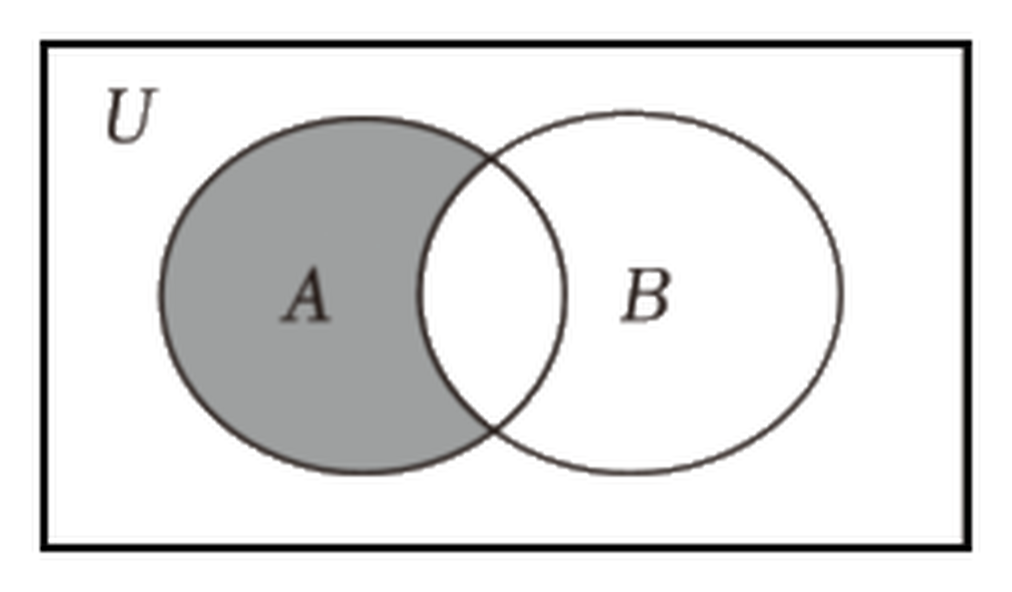
\includegraphics[width=0.34\textwidth]{figures/venn_A_minus_B.png}
\end{center}

\ans{$\{0,1,2\}$}

\ifanswer
\solbegin
\step{图中阴影部分表示的集合为 $A\cap\overline{B}=\{0,1,2\}$.}
\solend

\fi

\item 集合 $\{(x,y)\mid x+2y=2,\ x,y\in\N\}$ 用列举法表示为 \blankline[4.4em].

\ans{$\{(0,1),(2,0)\}$}

\ifanswer
\solbegin
\step{由题意得 $x+2y=2$ 可化为 $y=1-\dfrac{x}{2}$，}
\step{由 $y\in\N$，有 $y=1-\dfrac{x}{2}\geqslant 0$，解得 $x\leqslant 2$，}
\step{又由 $x\in\N$，得 $x$ 可能取值为 $0$，$1$，$2$，}
\step{当 $x=0$ 时，得 $y=1$，满足条件，}
\step{当 $x=1$ 时，得 $y=\dfrac{1}{2}\notin\N$，不满足条件，}
\step{当 $x=2$ 时，得 $y=0$，满足条件，}
\step{综上，集合用列举法表示为 $\{(0,1),(2,0)\}$.}
\solend

\fi

\item 若 $A=\{x\mid x=a^2+2a+4,\ a\in\R\}$，$B=\{y\mid y=b^2-4b+3,\ b\in\R\}$，则 $A$ 与 $B$ 的关系为 \blankline[4.4em].

% 注：此处符号为 $\subset$（真包含，无下划线；与第 10 题②、第 12 题、第 17 题等的
%     带下划线 $\subseteq$ 在卷面上明显不同，已逐处放大比对确认）。
\ans{$A\subset B$}

\ifanswer
\solbegin
\step{由 $x=a^2+2a+4=(a+1)^2+3$，}
\step{所以 $x=(a+1)^2+3\geqslant 3$，因此 $A=[3,+\infty)$，}
\step{由 $y=b^2-4b+3=(b-2)^2-1$，因为 $b\in\R$，所以 $y=(b-2)^2-1\geqslant -1$，}
\step{因此 $B=[-1,+\infty)$，因此 $A\subset B$.}
\solend

\fi

\item 在用反证法证明某命题时，对结论“$a,b,c$ 至少有一个为整数”的否定为 \blankline[4.4em].

\ans{$a,b,c$ 都不是整数}

\item 下列命题：①合数一定是偶数，②若 $A\cup B=B$，则 $A\sub B$，③方程 $ax+1=0$ 的解是 $x=-\dfrac{1}{a}$，④“$ac=bc$”是“$a=b$”的必要非充分条件，其中真命题的是 \blankline[2.4em]（填写序号）.

\ans{②④}

\ifanswer
\solbegin
% 注：以下 ①、③ 两行原卷印作「①为真命题」「③为真命题」，与两行自己给出的反例以及本段
%     末句「故真命题的是②④」都矛盾，系原卷笔误；本稿按文意订正为「为假命题」（结论不变）。
\step{对于①，$9$ 是合数，不是偶数，①为假命题；}
\step{对于②，由 $A\cup B=B$，得 $A\sub B$，②为真命题；}
\step{对于③，当 $a=0$ 时，$ax+1=0$ 无解，③为假命题；}
\step{对于④，当 $c=0$，$a=1$，$b=2$ 时满足 $ac=bc$，但 $a\neq b$，}
\step{当 $a=b$ 时，得 $ac=bc$，则“$ac=bc$”是“$a=b$”的必要非充分条件，}
\step{④为真命题.}
\step{故真命题的是②④.}
\solend

\fi

\item 设 $\alpha:4\leqslant x\leqslant 8$，$\beta:m+1\leqslant x\leqslant 2m+4$，$m\in\R$，$\alpha$ 是 $\beta$ 的充分不必要条件，则实数 $m$ 的取值范围是 \blankline[4.4em].

\ans{$[2,3]$}

\ifanswer
\solbegin
\step{因为 $\alpha$ 是 $\beta$ 的充分不必要条件，所以 $\begin{cases}m+1\leqslant 4\\ 2m+4\geqslant 8\end{cases}$，且等号不能同时成立，}
\step{解得 $2\leqslant m\leqslant 3$，所以实数 $m$ 的取值范围是 $[2,3]$.}
\solend

\fi

\item 已知集合 $A=\{a_1,a_2,\cdots,a_7\}$ 且 $A\sub\R$，定义 $\varphi(A)=\{a_ia_j\mid a_i,a_j\in A,\ 1\leqslant i<j\leqslant 7\}$，则 $\varphi(A)$ 的元素个数的最小值是 \blankline[2.4em].

\ans{$9$}

\ifanswer
\solbegin
\step{考虑等比数列，取 $A=\{-4,-2,-1,0,1,2,4\}$，}
\step{$\varphi(A)=\{8,4,0,-4,-8,-16,2,-2,-1\}$，元素个数最小值是 $9$.}
\solend

\fi

\end{enumerate}

\bigsec{二、选择题}

\begin{enumerate}
\setcounter{enumi}{12}

\item 已知 $M=\{(x,y)\mid x=y,\ x\in\R\}$，$N=\{(x,y)\mid y=x^2,\ x\in\R\}$，则 $M\cap N=$（\quad）.

A. $\{x\mid x\geqslant 0\}$\qquad B. $\{x\mid x\in\R\}$\qquad C. $\{(1,1)\}$\qquad D. $\{(1,1),(0,0)\}$

\ans{D}

\ifanswer
\solbegin
\step{联立方程组 $\begin{cases}x=y\\ y=x^2\end{cases}$，解得 $\begin{cases}x=0\\ y=0\end{cases}$ 或 $\begin{cases}x=1\\ y=1\end{cases}$，}
\step{则交点为 $(1,1)$、$(0,0)$，得到 $M\cap N=\{(1,1),(0,0)\}$. 故选 D.}
\solend

\fi

\item 下列说法中，正确的是（\quad）.

A. “$x>1$ 或 $y>1$”的否定形式是“$x\leqslant 1$ 或 $y\leqslant 1$”

B. “$1<x<3$”的否定形式是“$x<1$ 或 $x>3$”

C. “$\triangle ABC$ 是锐角三角形”的否定形式是“$\triangle ABC$ 中存在一个内角大于 $90^\circ$”

D. “任意 $x\in\R$，$f(x)=f(-x)$”的否定形式是“存在 $x_0\in\R$，使得 $f(x_0)\neq f(-x_0)$”

\ans{D}

\item 已知 $m,n$ 是非零自然数，命题 $\alpha:mn$ 是奇数，命题 $\beta:m$ 或 $n$ 是奇数，则 $\alpha$ 是 $\beta$ 的（\quad）

A. 充分非必要条件\qquad B. 必要非充分条件

C. 充要条件\qquad D. 既非充分又非必要条件

\ans{A}

\ifanswer
\solbegin
\step{$mn$ 是奇数 $\Leftrightarrow$ $m$、$n$ 都是奇数，所以 $\alpha$ 能推出 $\beta$，充分性成立，}
\step{但 $\beta$ 推不出 $\alpha$，必要性不成立，所以 $\alpha$ 是 $\beta$ 的充分非必要条件. 故选 A.}
\solend

\fi

\item 设 $k\geqslant 1,k\in\N$，已知集合 $M=\{1,2,3,4,5\}$，若集合 $N_1,N_2,\cdots,N_k$ 是集合 $M$ 的 $k$ 个不同非空子集，且 $N_1\cup N_2\cup\cdots\cup N_k\neq M$，则 $k$ 的最大值为（\quad）

A. $15$\qquad B. $16$\qquad C. $31$\qquad D. $32$

\ans{A}

\ifanswer
\solbegin
\step{由 $N_1\cup N_2\cup\cdots\cup N_k\neq M$ 得所有非空子集的并集缺少集合 $M$ 中至少一个元素，}
\step{假设缺少元素 $1$，则所有非空子集 $N_i$ 均不含元素 $1$，}
\step{即 $N_i$ 是集合 $\{2,3,4,5\}$ 非空子集，集合 $\{2,3,4,5\}$ 的非空子集个数为 $2^4-1=15$，}
\step{且这些子集 $N_i$ 的并集必不含 $1$，满足条件.}
\step{假设 $k\geqslant 16$，要满足所有非空子集的并集不等于集合 $M$，}
\step{必须至少有一个集合 $M$ 中的元素不在任何一个子集中，否则并集就会等于 $M$，}
\step{设这个缺失的元素是 $1$，那么 $k$ 个非空子集都不含元素 $1$，}
\step{即每个子集都是集合 $\{2,3,4,5\}$ 的非空子集，}
\step{而集合 $\{2,3,4,5\}$ 只有 $2^4-1=15$ 个不同的非空子集，}
\step{所以无法从中取出至少 $16$ 个不同的非空子集，}
\step{因此假设不成立，$k$ 必须小于 $16$，所以 $k$ 的最大值为 $15$，故选 A.}
\solend

\fi

\end{enumerate}

\bigsec{三、解答题}

\begin{enumerate}
\setcounter{enumi}{16}

\item 已知集合 $A=\{x\mid m-1\leqslant x\leqslant m+1\},B=\{x\mid x\leqslant 4\}$.

\begin{enumerate}[label=(\arabic*)]
\item 当 $m=4$ 时，求集合 $A\cap\overline{B}$；
\item 若“$x\in A$”是“$x\in B$”成立的充分非必要条件，求实数 $m$ 的取值范围.
\end{enumerate}

\ans{(1) $\{x\mid 4<x\leqslant 5\}$；（2）$\{m\mid m\leqslant 3\}$}

\ifanswer
\solbegin
\stepm{(1)}{当 $m=4$ 时，$A=\{x\mid 3\leqslant x\leqslant 5\}$，$\overline{B}=\{x\mid x>4\}$，}
\step{所以 $A\cap\overline{B}=\{x\mid 4<x\leqslant 5\}$.}
\stepm{(2)}{因为“$x\in A$”是“$x\in B$”成立的充分非必要条件，}
\step{所以 $A\sub B$，且 $B\neq A$，}
\step{易得 $A=\{x\mid m-1\leqslant x\leqslant m+1\}\neq\varnothing$，所以 $m+1\leqslant 4$，解得 $m\leqslant 3$，}
\step{符合题意；}
\step{综上所述，$m$ 的取值范围为 $\{m\mid m\leqslant 3\}$.}
\solend

\fi

\ansspace[7]

\item 设 $x\in\Z,a=x+5,b=20-x$.

\begin{enumerate}[label=(\arabic*)]
\item 求证：$a\neq b$；
\item 若 $c\in\Z$，求证：$c+a,c+b$ 中至少有一个数是奇数.
\end{enumerate}

\ans{(1) 略；（2）略}

\ifanswer
\solbegin
\stepm{(1)}{假设 $a=b$，则 $x+5=20-x\Rightarrow x=\dfrac{15}{2}\notin\Z$，与 $x\in\Z$ 矛盾，}
\step{则假设不成立，故 $a\neq b$.}
\stepm{(2)}{假设 $c+a,c+b$ 中都是偶数，}
\step{则 $c+a=c+x+5=2k_1,c+b=c+20-x=2k_2$，}
\step{两式相加并整理，得 $c=k_1+k_2-\dfrac{25}{2}\notin\Z$，与 $c\in\Z$ 矛盾，故假设不成立，}
\step{则 $c+a,c+b$ 中至少有一个数是奇数.}
\solend

\fi

\ansspace[8]

\item 设集合 $A=\{x\mid x^2+4x=0\}$，$B=\{x\mid x^2+2(a+1)x+a^2-1=0\}$.

\begin{enumerate}[label=(\arabic*)]
\item 写出集合 $A$ 的所有子集；
\item 若 $A\cap B=B$，求实数 $a$ 的取值范围.
\end{enumerate}

\ans{(1) $\varnothing,\{0\},\{-4\},\{0,-4\}$；（2）$a=1$ 或 $a\leqslant -1$}

\ifanswer
\solbegin
% 注：原卷此处列举子集时印作「$\{0-4\}$」，漏排逗号，本稿写作 $\{0,-4\}$.
\stepm{(1)}{由题意得 $A=\{0,-4\}$，集合 $A$ 的所有子集为 $\varnothing,\{0\},\{-4\},\{0,-4\}$；}
\stepm{(2)}{由 $A\cap B=B$ 得 $B\sub A$，}
\step{所以 $B=\{0\}$ 或 $B=\{-4\}$ 或 $B=\{0,-4\}$ 或 $B=\varnothing$，}
% 注：下面 $B=\{0\}$ 一行的两根之积，原卷印作 $a^2-1=-4\times(-4)$（与再下一行 $B=\{-4\}$
%     一字不差），按两根均为 0 之积应为 0；且原卷紧随的「解得 $a=-1$」也只在 $a^2-1=0$ 下成立，
%     故本稿订正为 $a^2-1=0$.
\step{若 $B=\{0\}$ 时，$x^2+2(a+1)x+a^2-1=0$ 有两个相等的根 $0$，}
\step{则 $\begin{cases}-2(a+1)=0\\ a^2-1=0\end{cases}$，解得 $a=-1$，}
\step{若 $B=\{-4\}$ 时，$x^2+2(a+1)x+a^2-1=0$ 有两个相等的根 $-4$，}
\step{则 $\begin{cases}-2(a+1)=-8\\ a^2-1=-4\times(-4)\end{cases}$，$a$ 无解，}
\step{若 $B=\{0,-4\}$ 时，$x^2+2(a+1)x+a^2-1=0$ 有两个不相等的根 $0$ 和 $-4$，}
\step{则 $\begin{cases}-2(a+1)=-4\\ a^2-1=0\end{cases}$，解得 $a=1$，}
\step{当 $B=\varnothing$ 时，$x^2+2(a+1)x+a^2-1=0$ 无实数根，}
\step{$\Delta=[2(a+1)]^2-4(a^2-1)=8a+8<0$，得 $a<-1$.}
\step{综上，$a=1$ 或 $a\leqslant -1$.}
\solend

\fi

\ansspace[8]

\item 已知集合 $A=\{x\mid x<-2\text{ 或 }x\geqslant 3\}$，$U=\R$.

\begin{enumerate}[label=(\arabic*)]
\item 求 $\overline{A}$；
\item 若 $B=\{x\mid mx-1>0\}$，当 $B\sub A$ 时，求实数 $m$ 的取值范围；
\item 若 $B=\{x\mid 2m-6\leqslant x\leqslant m+4\}$，当 $B\cap\overline{A}=\varnothing$ 时，求实数 $m$ 的取值范围.
\end{enumerate}

\ans{(1) $\{x\mid -2\leqslant x<3\}$；（2）$\left[-\dfrac{1}{2},\dfrac{1}{3}\right]$；（3）$(-\infty,-6)\cup\left[\dfrac{9}{2},+\infty\right)$}

\ifanswer
\solbegin
\stepm{(1)}{因为集合 $A=\{x\mid x<-2\text{ 或 }x\geqslant 3\}$，$U=\R$，所以 $\overline{A}=\{x\mid -2\leqslant x<3\}$；}
\stepm{(2)}{当 $m=0$ 时，$B=\varnothing$，符合题意，}
\step{当 $m>0$ 时，$B=\left\{x\mid x>\dfrac{1}{m}\right\}$，则 $\dfrac{1}{m}\geqslant 3$，解得 $0<m\leqslant\dfrac{1}{3}$，}
\step{当 $m<0$ 时，$B=\left\{x\mid x<\dfrac{1}{m}\right\}$，则 $\dfrac{1}{m}\leqslant -2$，解得 $-\dfrac{1}{2}\leqslant m<0$，}
\step{综上所述，实数 $m$ 的取值范围 $\left[-\dfrac{1}{2},\dfrac{1}{3}\right]$；}
\stepm{(3)}{由题意得 $B=\{x\mid 2m-6\leqslant x\leqslant m+4\}$，$\overline{A}=\{x\mid -2\leqslant x<3\}$，且 $B\cap\overline{A}=\varnothing$，}
\step{当 $B=\varnothing$ 时，$2m-6>m+4$，解得 $m>10$，}
\step{当 $B\neq\varnothing$ 时，则 $\begin{cases}2m-6\leqslant m+4\\ m+4<-2\end{cases}$ 或 $\begin{cases}2m-6\leqslant m+4\\ 2m-6\geqslant 3\end{cases}$，}
\step{解得 $m<-6$ 或 $\dfrac{9}{2}\leqslant m\leqslant 10$，}
\step{综上所述，实数 $m$ 的取值范围为 $(-\infty,-6)\cup\left[\dfrac{9}{2},+\infty\right)$.}
\solend

\fi

\ansspace[10]

% 压轴题：其后已无内容，故作答区全用可丢弃胶水（\ansspace*），并在题目前先量一下版面。
\ansneed{7cm}

\item 给定数集 $M$，若对于任意 $a$、$b\in M$，有 $a+b\in M,a-b\in M$，则称集合 $M$ 为闭集合.

\begin{enumerate}[label=(\arabic*)]
\item 判断集合 $A_1=\{-4,-2,0,2,4\}$，集合 $B=\{x\mid x=3k,k\in\Z\}$ 是否为闭集合；
\item 若集合 $C$、$D$ 为闭集合，则 $C\cup D$ 是否一定为闭集合？请说明理由；
\item 已知集合 $C$、$D$ 为闭集合，且 $C\subset\R,D\subset\R$，证明：$(C\cup D)\subset\R$.
\end{enumerate}

\ans{(1) $A_1$ 不是闭集合，$B$ 是闭集合；（2）不一定；（3）略}

\ifanswer
\solbegin
\stepm{(1)}{因为 $4\in A_1,2\in A_1,4+2=6\notin A_1$，所以 $A_1$ 不是闭集合；}
\step{任取 $x,y\in B$，设 $x=3m,y=3n,m,n\in\Z$，}
\step{则 $x+y=3m+3n=3(m+n)$ 且 $m+n\in\Z$，}
\step{所以 $x+y\in B$，同理，$x-y\in B$，故 $B$ 为闭集合.}
\stepm{(2)}{结论：不一定.}
\step{不妨令 $C=\{x\mid x=2k,k\in\Z\},D=\{x\mid x=3k,k\in\Z\}$，}
\step{则由（1）得 $C$、$D$ 为闭集合，易得 $2,3\in C\cup D,2+3=5\notin C\cup D$，}
\step{因此，$C\cup D$ 不一定是闭集合.}
\stepm{(3)}{不妨假设 $C\cup D=\R$，则由 $C\subset\R$，得存在 $a\in\R$ 且 $a\notin C$，故 $a\in D$.}
\step{同理，存在 $b\in\R$ 且 $b\notin D$，故 $b\in C$.}
\step{因为 $a+b\in\R=C\cup D$，所以 $a+b\in C$ 或 $a+b\in D$.}
\step{若 $a+b\in C$，则由 $C$ 为闭集合且 $b\in C$，得 $a=(a+b)-b\in C$，}
\step{与 $a\notin C$ 矛盾.}
\step{若 $a+b\in D$，则由 $D$ 为闭集合且 $a\in D$，得 $b=(a+b)-a\in D$，}
\step{与 $b\notin D$ 矛盾.}
\step{综上，$C\cup D=\R$ 不成立，故 $(C\cup D)\subset\R$.}
\solend

\fi

\ansspace*[12]

\end{enumerate}

\end{document}
"
%
% 原始材料是微信公众号图文（公众号「破晓」），正文为 7 张 PNG 页；原文本身就是一份**讲评版**
% ——题目下方直接印出【答案】或【解析】。试题文字、答案与解析均照原卷录入，未改内容。
%
% 与原卷的排版差异（均已在 README「说明」中交代）：
%   ① 原文自**第 3 题**起（第 1、2 题未在该文中发布），故本稿题号亦自 3 起；
%   ② 原卷未印分节标题，本稿按题型补「一、填空题 / 二、选择题 / 三、解答题」三节；
%   ③ 原卷填空、选择的答案直接印在题目下方（第 14 题更是直接印在括注里），本稿统一改为
%      试卷版隐去、答案版以【答案】给出，使两版彻底分离；
%   ④ 原卷的实数集符号时作正体 $R$、时作粗体 $\mathbf{R}$（第 14 题 D 选项与第 21 题均为粗体），
%      本稿按全稿惯例统一写作 $\R$.
%
% 原卷笔误三处（已逐处放大到能看清字形后核对，本稿按文意订正，并在 README 中写明原委）：
%   ① 第 10 题【解析】①、③ 两行原卷印作「①为真命题」「③为真命题」，与同段结论
%      「故真命题的是②④」以及两行自己给出的反例（9 是合数却不是偶数；$a=0$ 时方程无解）
%      都矛盾，显系笔误，本稿订正为「为假命题」；
%   ② 第 19(2) 中 $B=\{0\}$ 一行原卷印作 $a^2-1=-4\times(-4)$（与下一行 $B=\{-4\}$ 一字不差），
%      按两根均为 0 之积应为 0，本稿订正为 $a^2-1=0$——原卷紧接的「解得 $a=-1$」也只在
%      $a^2-1=0$ 下成立（注：同一道题在《高一07 交附闵行周练1》中原样抄录，此处按文意订正）；
%   ③ 第 19(1)【解析】列举子集时原卷印作「$\{0-4\}$」，漏排逗号，本稿写作 $\{0,-4\}$.

\documentclass[a4paper,11pt]{article}
\usepackage{common}

\begin{document}

\examtitlest[3]{2026--2027 年复附浦东高一上周末作业 2}{集合与常用逻辑用语}

\bigsec{一、填空题}

\begin{enumerate}
\setcounter{enumi}{2}

\item 已知集合 $A=\{2,a\}$，且 $1\in A$，则 $a=$ \blankline[2.4em].

\ans{$1$}

\item 集合 $A=\{x\mid x^2=1\}$，$B=\{x\mid x^2+x=0\}$，则 $A\cap B=$ \blankline[4.4em].

\ans{$\{-1\}$}

\ifanswer
\solbegin
\step{集合 $A=\{x\mid x^2=1\}=\{-1,1\}$，$B=\{x\mid x^2+x=0\}=\{-1,0\}$，}
\step{由交集定义得 $A\cap B=\{-1\}$.}
\solend

\fi

\item 已知集合 $A=\{1,3,5\},B=\{2,3,6\}$，则 $A\cup B=$ \blankline[4.4em].

\ans{$\{1,2,3,5,6\}$}

\item 若全集 $U=\R$，集合 $A=\{0,1,2,3,4\}$，$B=\{x\mid x>2\}$，则右图中阴影部分表示的集合为 \blankline[4.4em].

\begin{center}
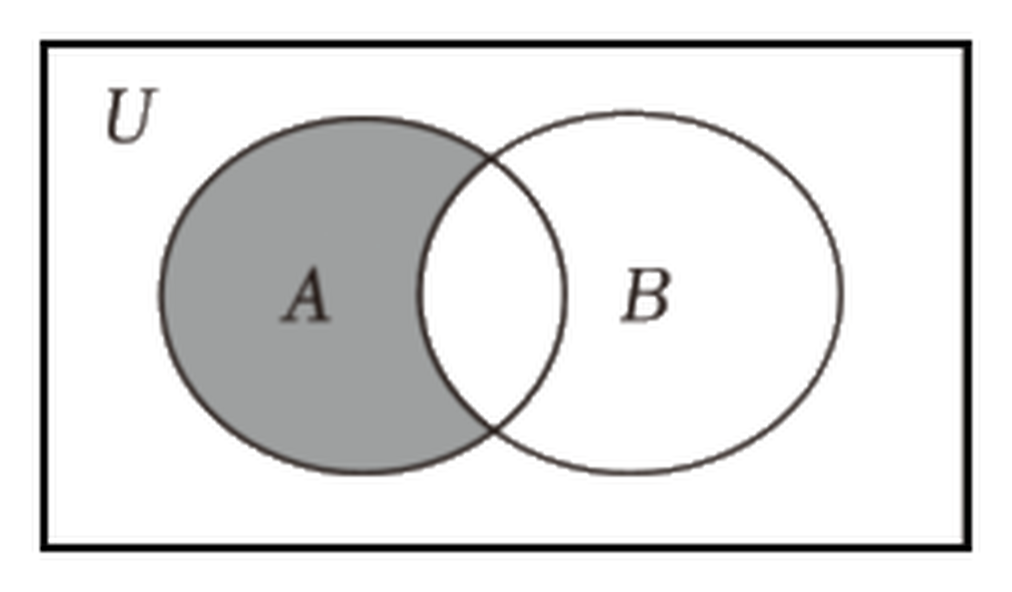
\includegraphics[width=0.34\textwidth]{figures/venn_A_minus_B.png}
\end{center}

\ans{$\{0,1,2\}$}

\ifanswer
\solbegin
\step{图中阴影部分表示的集合为 $A\cap\overline{B}=\{0,1,2\}$.}
\solend

\fi

\item 集合 $\{(x,y)\mid x+2y=2,\ x,y\in\N\}$ 用列举法表示为 \blankline[4.4em].

\ans{$\{(0,1),(2,0)\}$}

\ifanswer
\solbegin
\step{由题意得 $x+2y=2$ 可化为 $y=1-\dfrac{x}{2}$，}
\step{由 $y\in\N$，有 $y=1-\dfrac{x}{2}\geqslant 0$，解得 $x\leqslant 2$，}
\step{又由 $x\in\N$，得 $x$ 可能取值为 $0$，$1$，$2$，}
\step{当 $x=0$ 时，得 $y=1$，满足条件，}
\step{当 $x=1$ 时，得 $y=\dfrac{1}{2}\notin\N$，不满足条件，}
\step{当 $x=2$ 时，得 $y=0$，满足条件，}
\step{综上，集合用列举法表示为 $\{(0,1),(2,0)\}$.}
\solend

\fi

\item 若 $A=\{x\mid x=a^2+2a+4,\ a\in\R\}$，$B=\{y\mid y=b^2-4b+3,\ b\in\R\}$，则 $A$ 与 $B$ 的关系为 \blankline[4.4em].

% 注：此处符号为 $\subset$（真包含，无下划线；与第 10 题②、第 12 题、第 17 题等的
%     带下划线 $\subseteq$ 在卷面上明显不同，已逐处放大比对确认）。
\ans{$A\subset B$}

\ifanswer
\solbegin
\step{由 $x=a^2+2a+4=(a+1)^2+3$，}
\step{所以 $x=(a+1)^2+3\geqslant 3$，因此 $A=[3,+\infty)$，}
\step{由 $y=b^2-4b+3=(b-2)^2-1$，因为 $b\in\R$，所以 $y=(b-2)^2-1\geqslant -1$，}
\step{因此 $B=[-1,+\infty)$，因此 $A\subset B$.}
\solend

\fi

\item 在用反证法证明某命题时，对结论“$a,b,c$ 至少有一个为整数”的否定为 \blankline[4.4em].

\ans{$a,b,c$ 都不是整数}

\item 下列命题：①合数一定是偶数，②若 $A\cup B=B$，则 $A\sub B$，③方程 $ax+1=0$ 的解是 $x=-\dfrac{1}{a}$，④“$ac=bc$”是“$a=b$”的必要非充分条件，其中真命题的是 \blankline[2.4em]（填写序号）.

\ans{②④}

\ifanswer
\solbegin
% 注：以下 ①、③ 两行原卷印作「①为真命题」「③为真命题」，与两行自己给出的反例以及本段
%     末句「故真命题的是②④」都矛盾，系原卷笔误；本稿按文意订正为「为假命题」（结论不变）。
\step{对于①，$9$ 是合数，不是偶数，①为假命题；}
\step{对于②，由 $A\cup B=B$，得 $A\sub B$，②为真命题；}
\step{对于③，当 $a=0$ 时，$ax+1=0$ 无解，③为假命题；}
\step{对于④，当 $c=0$，$a=1$，$b=2$ 时满足 $ac=bc$，但 $a\neq b$，}
\step{当 $a=b$ 时，得 $ac=bc$，则“$ac=bc$”是“$a=b$”的必要非充分条件，}
\step{④为真命题.}
\step{故真命题的是②④.}
\solend

\fi

\item 设 $\alpha:4\leqslant x\leqslant 8$，$\beta:m+1\leqslant x\leqslant 2m+4$，$m\in\R$，$\alpha$ 是 $\beta$ 的充分不必要条件，则实数 $m$ 的取值范围是 \blankline[4.4em].

\ans{$[2,3]$}

\ifanswer
\solbegin
\step{因为 $\alpha$ 是 $\beta$ 的充分不必要条件，所以 $\begin{cases}m+1\leqslant 4\\ 2m+4\geqslant 8\end{cases}$，且等号不能同时成立，}
\step{解得 $2\leqslant m\leqslant 3$，所以实数 $m$ 的取值范围是 $[2,3]$.}
\solend

\fi

\item 已知集合 $A=\{a_1,a_2,\cdots,a_7\}$ 且 $A\sub\R$，定义 $\varphi(A)=\{a_ia_j\mid a_i,a_j\in A,\ 1\leqslant i<j\leqslant 7\}$，则 $\varphi(A)$ 的元素个数的最小值是 \blankline[2.4em].

\ans{$9$}

\ifanswer
\solbegin
\step{考虑等比数列，取 $A=\{-4,-2,-1,0,1,2,4\}$，}
\step{$\varphi(A)=\{8,4,0,-4,-8,-16,2,-2,-1\}$，元素个数最小值是 $9$.}
\solend

\fi

\end{enumerate}

\bigsec{二、选择题}

\begin{enumerate}
\setcounter{enumi}{12}

\item 已知 $M=\{(x,y)\mid x=y,\ x\in\R\}$，$N=\{(x,y)\mid y=x^2,\ x\in\R\}$，则 $M\cap N=$（\quad）.

A. $\{x\mid x\geqslant 0\}$\qquad B. $\{x\mid x\in\R\}$\qquad C. $\{(1,1)\}$\qquad D. $\{(1,1),(0,0)\}$

\ans{D}

\ifanswer
\solbegin
\step{联立方程组 $\begin{cases}x=y\\ y=x^2\end{cases}$，解得 $\begin{cases}x=0\\ y=0\end{cases}$ 或 $\begin{cases}x=1\\ y=1\end{cases}$，}
\step{则交点为 $(1,1)$、$(0,0)$，得到 $M\cap N=\{(1,1),(0,0)\}$. 故选 D.}
\solend

\fi

\item 下列说法中，正确的是（\quad）.

A. “$x>1$ 或 $y>1$”的否定形式是“$x\leqslant 1$ 或 $y\leqslant 1$”

B. “$1<x<3$”的否定形式是“$x<1$ 或 $x>3$”

C. “$\triangle ABC$ 是锐角三角形”的否定形式是“$\triangle ABC$ 中存在一个内角大于 $90^\circ$”

D. “任意 $x\in\R$，$f(x)=f(-x)$”的否定形式是“存在 $x_0\in\R$，使得 $f(x_0)\neq f(-x_0)$”

\ans{D}

\item 已知 $m,n$ 是非零自然数，命题 $\alpha:mn$ 是奇数，命题 $\beta:m$ 或 $n$ 是奇数，则 $\alpha$ 是 $\beta$ 的（\quad）

A. 充分非必要条件\qquad B. 必要非充分条件

C. 充要条件\qquad D. 既非充分又非必要条件

\ans{A}

\ifanswer
\solbegin
\step{$mn$ 是奇数 $\Leftrightarrow$ $m$、$n$ 都是奇数，所以 $\alpha$ 能推出 $\beta$，充分性成立，}
\step{但 $\beta$ 推不出 $\alpha$，必要性不成立，所以 $\alpha$ 是 $\beta$ 的充分非必要条件. 故选 A.}
\solend

\fi

\item 设 $k\geqslant 1,k\in\N$，已知集合 $M=\{1,2,3,4,5\}$，若集合 $N_1,N_2,\cdots,N_k$ 是集合 $M$ 的 $k$ 个不同非空子集，且 $N_1\cup N_2\cup\cdots\cup N_k\neq M$，则 $k$ 的最大值为（\quad）

A. $15$\qquad B. $16$\qquad C. $31$\qquad D. $32$

\ans{A}

\ifanswer
\solbegin
\step{由 $N_1\cup N_2\cup\cdots\cup N_k\neq M$ 得所有非空子集的并集缺少集合 $M$ 中至少一个元素，}
\step{假设缺少元素 $1$，则所有非空子集 $N_i$ 均不含元素 $1$，}
\step{即 $N_i$ 是集合 $\{2,3,4,5\}$ 非空子集，集合 $\{2,3,4,5\}$ 的非空子集个数为 $2^4-1=15$，}
\step{且这些子集 $N_i$ 的并集必不含 $1$，满足条件.}
\step{假设 $k\geqslant 16$，要满足所有非空子集的并集不等于集合 $M$，}
\step{必须至少有一个集合 $M$ 中的元素不在任何一个子集中，否则并集就会等于 $M$，}
\step{设这个缺失的元素是 $1$，那么 $k$ 个非空子集都不含元素 $1$，}
\step{即每个子集都是集合 $\{2,3,4,5\}$ 的非空子集，}
\step{而集合 $\{2,3,4,5\}$ 只有 $2^4-1=15$ 个不同的非空子集，}
\step{所以无法从中取出至少 $16$ 个不同的非空子集，}
\step{因此假设不成立，$k$ 必须小于 $16$，所以 $k$ 的最大值为 $15$，故选 A.}
\solend

\fi

\end{enumerate}

\bigsec{三、解答题}

\begin{enumerate}
\setcounter{enumi}{16}

\item 已知集合 $A=\{x\mid m-1\leqslant x\leqslant m+1\},B=\{x\mid x\leqslant 4\}$.

\begin{enumerate}[label=(\arabic*)]
\item 当 $m=4$ 时，求集合 $A\cap\overline{B}$；
\item 若“$x\in A$”是“$x\in B$”成立的充分非必要条件，求实数 $m$ 的取值范围.
\end{enumerate}

\ans{(1) $\{x\mid 4<x\leqslant 5\}$；（2）$\{m\mid m\leqslant 3\}$}

\ifanswer
\solbegin
\stepm{(1)}{当 $m=4$ 时，$A=\{x\mid 3\leqslant x\leqslant 5\}$，$\overline{B}=\{x\mid x>4\}$，}
\step{所以 $A\cap\overline{B}=\{x\mid 4<x\leqslant 5\}$.}
\stepm{(2)}{因为“$x\in A$”是“$x\in B$”成立的充分非必要条件，}
\step{所以 $A\sub B$，且 $B\neq A$，}
\step{易得 $A=\{x\mid m-1\leqslant x\leqslant m+1\}\neq\varnothing$，所以 $m+1\leqslant 4$，解得 $m\leqslant 3$，}
\step{符合题意；}
\step{综上所述，$m$ 的取值范围为 $\{m\mid m\leqslant 3\}$.}
\solend

\fi

\ansspace[7]

\item 设 $x\in\Z,a=x+5,b=20-x$.

\begin{enumerate}[label=(\arabic*)]
\item 求证：$a\neq b$；
\item 若 $c\in\Z$，求证：$c+a,c+b$ 中至少有一个数是奇数.
\end{enumerate}

\ans{(1) 略；（2）略}

\ifanswer
\solbegin
\stepm{(1)}{假设 $a=b$，则 $x+5=20-x\Rightarrow x=\dfrac{15}{2}\notin\Z$，与 $x\in\Z$ 矛盾，}
\step{则假设不成立，故 $a\neq b$.}
\stepm{(2)}{假设 $c+a,c+b$ 中都是偶数，}
\step{则 $c+a=c+x+5=2k_1,c+b=c+20-x=2k_2$，}
\step{两式相加并整理，得 $c=k_1+k_2-\dfrac{25}{2}\notin\Z$，与 $c\in\Z$ 矛盾，故假设不成立，}
\step{则 $c+a,c+b$ 中至少有一个数是奇数.}
\solend

\fi

\ansspace[8]

\item 设集合 $A=\{x\mid x^2+4x=0\}$，$B=\{x\mid x^2+2(a+1)x+a^2-1=0\}$.

\begin{enumerate}[label=(\arabic*)]
\item 写出集合 $A$ 的所有子集；
\item 若 $A\cap B=B$，求实数 $a$ 的取值范围.
\end{enumerate}

\ans{(1) $\varnothing,\{0\},\{-4\},\{0,-4\}$；（2）$a=1$ 或 $a\leqslant -1$}

\ifanswer
\solbegin
% 注：原卷此处列举子集时印作「$\{0-4\}$」，漏排逗号，本稿写作 $\{0,-4\}$.
\stepm{(1)}{由题意得 $A=\{0,-4\}$，集合 $A$ 的所有子集为 $\varnothing,\{0\},\{-4\},\{0,-4\}$；}
\stepm{(2)}{由 $A\cap B=B$ 得 $B\sub A$，}
\step{所以 $B=\{0\}$ 或 $B=\{-4\}$ 或 $B=\{0,-4\}$ 或 $B=\varnothing$，}
% 注：下面 $B=\{0\}$ 一行的两根之积，原卷印作 $a^2-1=-4\times(-4)$（与再下一行 $B=\{-4\}$
%     一字不差），按两根均为 0 之积应为 0；且原卷紧随的「解得 $a=-1$」也只在 $a^2-1=0$ 下成立，
%     故本稿订正为 $a^2-1=0$.
\step{若 $B=\{0\}$ 时，$x^2+2(a+1)x+a^2-1=0$ 有两个相等的根 $0$，}
\step{则 $\begin{cases}-2(a+1)=0\\ a^2-1=0\end{cases}$，解得 $a=-1$，}
\step{若 $B=\{-4\}$ 时，$x^2+2(a+1)x+a^2-1=0$ 有两个相等的根 $-4$，}
\step{则 $\begin{cases}-2(a+1)=-8\\ a^2-1=-4\times(-4)\end{cases}$，$a$ 无解，}
\step{若 $B=\{0,-4\}$ 时，$x^2+2(a+1)x+a^2-1=0$ 有两个不相等的根 $0$ 和 $-4$，}
\step{则 $\begin{cases}-2(a+1)=-4\\ a^2-1=0\end{cases}$，解得 $a=1$，}
\step{当 $B=\varnothing$ 时，$x^2+2(a+1)x+a^2-1=0$ 无实数根，}
\step{$\Delta=[2(a+1)]^2-4(a^2-1)=8a+8<0$，得 $a<-1$.}
\step{综上，$a=1$ 或 $a\leqslant -1$.}
\solend

\fi

\ansspace[8]

\item 已知集合 $A=\{x\mid x<-2\text{ 或 }x\geqslant 3\}$，$U=\R$.

\begin{enumerate}[label=(\arabic*)]
\item 求 $\overline{A}$；
\item 若 $B=\{x\mid mx-1>0\}$，当 $B\sub A$ 时，求实数 $m$ 的取值范围；
\item 若 $B=\{x\mid 2m-6\leqslant x\leqslant m+4\}$，当 $B\cap\overline{A}=\varnothing$ 时，求实数 $m$ 的取值范围.
\end{enumerate}

\ans{(1) $\{x\mid -2\leqslant x<3\}$；（2）$\left[-\dfrac{1}{2},\dfrac{1}{3}\right]$；（3）$(-\infty,-6)\cup\left[\dfrac{9}{2},+\infty\right)$}

\ifanswer
\solbegin
\stepm{(1)}{因为集合 $A=\{x\mid x<-2\text{ 或 }x\geqslant 3\}$，$U=\R$，所以 $\overline{A}=\{x\mid -2\leqslant x<3\}$；}
\stepm{(2)}{当 $m=0$ 时，$B=\varnothing$，符合题意，}
\step{当 $m>0$ 时，$B=\left\{x\mid x>\dfrac{1}{m}\right\}$，则 $\dfrac{1}{m}\geqslant 3$，解得 $0<m\leqslant\dfrac{1}{3}$，}
\step{当 $m<0$ 时，$B=\left\{x\mid x<\dfrac{1}{m}\right\}$，则 $\dfrac{1}{m}\leqslant -2$，解得 $-\dfrac{1}{2}\leqslant m<0$，}
\step{综上所述，实数 $m$ 的取值范围 $\left[-\dfrac{1}{2},\dfrac{1}{3}\right]$；}
\stepm{(3)}{由题意得 $B=\{x\mid 2m-6\leqslant x\leqslant m+4\}$，$\overline{A}=\{x\mid -2\leqslant x<3\}$，且 $B\cap\overline{A}=\varnothing$，}
\step{当 $B=\varnothing$ 时，$2m-6>m+4$，解得 $m>10$，}
\step{当 $B\neq\varnothing$ 时，则 $\begin{cases}2m-6\leqslant m+4\\ m+4<-2\end{cases}$ 或 $\begin{cases}2m-6\leqslant m+4\\ 2m-6\geqslant 3\end{cases}$，}
\step{解得 $m<-6$ 或 $\dfrac{9}{2}\leqslant m\leqslant 10$，}
\step{综上所述，实数 $m$ 的取值范围为 $(-\infty,-6)\cup\left[\dfrac{9}{2},+\infty\right)$.}
\solend

\fi

\ansspace[10]

% 压轴题：其后已无内容，故作答区全用可丢弃胶水（\ansspace*），并在题目前先量一下版面。
\ansneed{7cm}

\item 给定数集 $M$，若对于任意 $a$、$b\in M$，有 $a+b\in M,a-b\in M$，则称集合 $M$ 为闭集合.

\begin{enumerate}[label=(\arabic*)]
\item 判断集合 $A_1=\{-4,-2,0,2,4\}$，集合 $B=\{x\mid x=3k,k\in\Z\}$ 是否为闭集合；
\item 若集合 $C$、$D$ 为闭集合，则 $C\cup D$ 是否一定为闭集合？请说明理由；
\item 已知集合 $C$、$D$ 为闭集合，且 $C\subset\R,D\subset\R$，证明：$(C\cup D)\subset\R$.
\end{enumerate}

\ans{(1) $A_1$ 不是闭集合，$B$ 是闭集合；（2）不一定；（3）略}

\ifanswer
\solbegin
\stepm{(1)}{因为 $4\in A_1,2\in A_1,4+2=6\notin A_1$，所以 $A_1$ 不是闭集合；}
\step{任取 $x,y\in B$，设 $x=3m,y=3n,m,n\in\Z$，}
\step{则 $x+y=3m+3n=3(m+n)$ 且 $m+n\in\Z$，}
\step{所以 $x+y\in B$，同理，$x-y\in B$，故 $B$ 为闭集合.}
\stepm{(2)}{结论：不一定.}
\step{不妨令 $C=\{x\mid x=2k,k\in\Z\},D=\{x\mid x=3k,k\in\Z\}$，}
\step{则由（1）得 $C$、$D$ 为闭集合，易得 $2,3\in C\cup D,2+3=5\notin C\cup D$，}
\step{因此，$C\cup D$ 不一定是闭集合.}
\stepm{(3)}{不妨假设 $C\cup D=\R$，则由 $C\subset\R$，得存在 $a\in\R$ 且 $a\notin C$，故 $a\in D$.}
\step{同理，存在 $b\in\R$ 且 $b\notin D$，故 $b\in C$.}
\step{因为 $a+b\in\R=C\cup D$，所以 $a+b\in C$ 或 $a+b\in D$.}
\step{若 $a+b\in C$，则由 $C$ 为闭集合且 $b\in C$，得 $a=(a+b)-b\in C$，}
\step{与 $a\notin C$ 矛盾.}
\step{若 $a+b\in D$，则由 $D$ 为闭集合且 $a\in D$，得 $b=(a+b)-a\in D$，}
\step{与 $b\notin D$ 矛盾.}
\step{综上，$C\cup D=\R$ 不成立，故 $(C\cup D)\subset\R$.}
\solend

\fi

\ansspace*[12]

\end{enumerate}

\end{document}
